\begin{sepframe}{Complexity}
    {\scriptsize{Simplicity is the ultimate sophistication. L. Da Vinci}}
\end{sepframe}

\begin{frame}
    \frametitle{Complexity}
    \framesubtitle{Complexity at a glance}

    \begin{itemize}[<+->]
        \item Used to compare algorithms efficiency,
        \item Often calculated using the worst case scenario,
        \item In big $\mathcal{O}$ notation: $\mathcal{O}(1)$, $\mathcal{O}(n)$, $\mathcal{O}(n \times log(n))$, $\mathcal{O}(n^2)$
    \end{itemize}

    \note[item]{
        Lets start with the first one, this is usually the most classical one
        when dealing with algorithms.
    }
\end{frame}

\begin{frame}
    \frametitle{Complexity}
    \framesubtitle{Types}

    \begin{itemize}[<+->]
        \item Time complexity
        \item Space complexity
        \item Kolmogorov complexity
        \item Cyclomatic complexity
    \end{itemize}

    \note[item]{
        How about now diving into the marvellous world of algorithmic
        complexity?
        Worry not! We are just going to scratch the surface, nothing fancy
        at all.
    }
    \note[item]{
        We are going to "explore" 4 complexity types. Here they are.
    }
    \note[item]{
        Lets start with the first one, this is usually the most classical one
        when dealing with algorithms.
    }
\end{frame}

\begin{frame}
    \frametitle{Complexity}
    \framesubtitle{Constant time complexity: $\mathcal{O}(1)$}
    \lstinputlisting{src/session/complexity/resources/time-complexity-constant.php}

    \note[item]{
        Let's explain the time complexity with some examples...
    }
    \note[item]{
        Here's the first one. Can you guess what this snippet is doing?
    }
    \note[item]{
        Well, here's the solution. This snippet is returning the first item
        of any type of iterable. If we had to measure its complexity, it would
        be $\mathcal{O}(1)$
    }
\end{frame}

\begin{frame}
    \frametitle{Complexity}
    \framesubtitle{Linear time complexity: $\mathcal{O}(n)$}
    \lstinputlisting{src/session/complexity/resources/time-complexity-linear.php}
    \note[item]{
        Well, here's the solution. This snippet is returning the first item
        of any type of iterable. If we had to measure its complexity, it would
        be $\mathcal{O}(n)$
    }
\end{frame}

\begin{frame}
    \frametitle{Complexity}
    \framesubtitle{Exponential time complexity: $\mathcal{O}(n^2)$}
    \lstinputlisting{src/session/complexity/resources/time-complexity-exp.php}
\end{frame}

\begin{frame}
    \frametitle{Complexity}
    \framesubtitle{Space complexity}
    \lstinputlisting{src/session/complexity/resources/space-complexity.php}
\end{frame}

\begin{frame}
    \frametitle{Complexity}
    \framesubtitle{Kolmogorov complexity}

    The Kolmogorov complexity is the shortest size of a program that yield the
    expected output.
\end{frame}

\begin{frame}
    \frametitle{Complexity}
    \framesubtitle{Kolmogorov complexity}

    Let the following strings:

    \pause

    \begin{scriptsize}
        \begin{itemize}[<+->]
            \item \texttt{1111111111111111111111111111111111111111111111111111111111111111}
            \item \texttt{317b773017df0ab62b15cd3f2ad17d7b13ab02f05f4943011ef8c4067d1ca0a5}
        \end{itemize}
    \end{scriptsize}

    \pause[\thebeamerpauses]

    \vfill

    Which one has the smallest algorithm yielding those strings?
\end{frame}

\begin{frame}
    \frametitle{Complexity}
    \framesubtitle{Kolmogorov complexity}

    \lstinputlisting{src/session/complexity/resources/kolmogorov-complexity-example1.php}
\end{frame}

\begin{frame}
    \frametitle{Complexity}
    \framesubtitle{Kolmogorov complexity}

    The Kolmogorov complexity is the generalization of Shannon's theory of
    information.
    \\
    It has links to many other fields like with Gödel's incompleteness
    theorem, Turing's halting problem, compression theory, ...
    \\
    \bigskip
     \pause
    ``\textit{There is no way to tell if the K complexity of an algorithm is the
    shortest one}''.
\end{frame}

\begin{frame}
    \frametitle{Complexity}
    \framesubtitle{Cyclomatic complexity}

    \lstinputlisting{src/session/introduction/resources/complexity-example.php}
\end{frame}

\begin{frame}[fragile,c]
    \frametitle{Complexity}
    \framesubtitle{Cyclomatic complexity}

    \makebox[\linewidth]{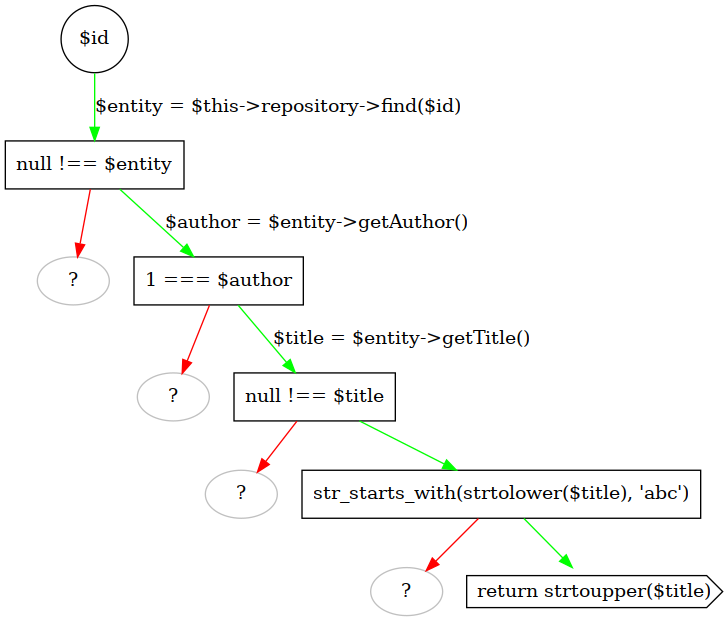
\includegraphics[height=.70\paperheight]{src/session/complexity/resources/complexity-example.png}}
\end{frame}

\begin{frame}[fragile,c]
    \frametitle{Complexity}
    \framesubtitle{Cyclomatic complexity}

    Conditions and type checks adds unnecessary complexity to a program,
    we are going to see how we can get rid of them.
\end{frame}

\begin{frame}[fragile,c]
    \frametitle{Complexity}
    \framesubtitle{Reducing the amount of nested conditions}

    But\pause\ but\pause\ but\pause ... we need conditions !
    \pause
    Of course.
\end{frame}

\begin{frame}[fragile,c]
    \frametitle{Complexity}
    \framesubtitle{Reducing the amount of nested conditions}

    EARLY RETURNS !
\end{frame}

\begin{frame}[fragile,c]
    \frametitle{Complexity}
    \framesubtitle{Cyclomatic complexity}

    \begin{lstlisting}[language=php]
    if ($expr1 && $expr2 && $expr3) {
        return true;
    }

    return false;
    \end{lstlisting}

    \pause

    is equivalent to:

    \begin{lstlisting}[language=php]
    if (! $expr1) {
        return false;
    }

    if (! $expr2) {
        return false;
    }

    if (! $expr3) {
        return false;
    }

    return true;
    \end{lstlisting}
\end{frame}

\begin{frame}
    \frametitle{Complexity}
    \framesubtitle{Cyclomatic complexity}

    \lstinputlisting{src/session/complexity/resources/complexity-example-early-returns.php}
\end{frame}

\begin{frame}
    \frametitle{Complexity}
    \framesubtitle{Cyclomatic complexity}

\lstinputlisting[caption={Imperative programming}]{src/session/complexity/resources/avoid-else1-a.js}
\pause
\lstinputlisting[caption={Declarative programming}]{src/session/complexity/resources/avoid-else1-b.js}
\end{frame}

\begin{frame}
    \frametitle{Complexity}
    \framesubtitle{Cyclomatic complexity}

    \begin{itemize}[<+->]
        \item Think to the ``\textcolor{red}{unhappy}'' paths at first
        \item The ``\textcolor{green}{happy}'' path, is usually the last line,
        \item Easier to read, understand,
        \item Longer to write.
    \end{itemize}
\end{frame}

\begin{frame}
    \frametitle{Complexity}
    \framesubtitle{Imperative programming}

    Imperative programming tells the machine how to do something.

    \pause

    (resulting in what you want to happen).
\end{frame}

\begin{frame}
    \frametitle{Complexity}
    \framesubtitle{Declarative programming}

    Declarative programming tells the machine what you would like to happen.

    \pause

    (and the computer figures out how to do it)
\end{frame}

\begin{frame}
    \frametitle{Complexity}
    \framesubtitle{Imperative and declarative programming}

\lstinputlisting[caption={Imperative programming}]{src/session/history/resources/oop.js}
\pause
\lstinputlisting[caption={Declarative programming}]{src/session/history/resources/fp.js}
\end{frame}

\begin{frame}
    \frametitle{Complexity}
    \framesubtitle{Imperative and declarative programming}

\lstinputlisting[caption={Imperative programming}]{src/session/complexity/resources/imperative1.js}
\pause
\lstinputlisting[caption={Declarative programming}]{src/session/complexity/resources/declarative1.js}
\end{frame}

\begin{frame}
    \frametitle{Complexity}
    \framesubtitle{Abstracting away the complexity?}

    Have you every wondered why there are so much packages existing for a
    particular languages?\\
    \pause
    Most probably they were created to fix particular and recurrent issues or
    boring problematic?\\
    \pause
    Sometimes it could be nice to query the language package managers to find if
    the solution to your problem doesn't already exists!\\
    \pause
    This would delegate the responsibility somewhere else and reduce the overall
    complexity of your application.\\
    \pause
    It is also less code to maintain and thus, less prone to bugs.
\end{frame}

\begin{frame}
    \frametitle{Complexity}
    \framesubtitle{Confidence in other packages?}

    Relying on someone else's code means a lot, for some reason people prefer
    redoing things on their own.\\
    \pause
    I believe that developers should be able to evaluate the trust into a
    package based on some key indicators.\\
    \pause
    Tests, popularity, code lisibility, code extensibility, code practices...
\end{frame}

\begin{frame}
    \frametitle{Complexity}
    \framesubtitle{Confidence in other packages?}

    This is the reason why when making a package, it's better to be as strict
    as possible so the developer using your code doesn't have any surprise when
    using your code in its own.\\
    \pause
    Avoid mixing types, throw proper exceptions in case of issues, etc etc.\\
    \pause
    Let's remind to the audience how to put those tips in practice.
\end{frame}
